\section{Introduction and Scope of Tutorials}

The WESTPA (Weighted Ensemble Simulation Toolkit with Parallelization and Analysis) software package is a highly scalable implementation of the weighted ensemble (WE) path sampling strategy \citep{huber_weighted-ensemble_1996,zuckerman_weighted_2017} that has helped transform what is feasible for molecular simulations in the generation of pathways for long-timescale processes (> µs) with rigorous kinetics.
Among these simulations are atomically detailed simulations of protein folding \citep{adhikari_computational_2019}, protein-protein binding \citep{saglam_proteinprotein_2019}, protein-ligand unbinding \citep{lotz_unbiased_2018}, and the large-scale opening of the SARS-CoV-2 spike protein \citep{sztain_glycan_2021}. 
The latter involved the slowest process (seconds-timescale) yet studied for a massive system (one million atoms) using WE simulations. 
As a “bleeding edge” application, these efforts have motivated major upgrades to WESTPA (version 2.0) that enable the sampling of processes at even longer timescales and more streamlined handling of large datasets \citep{russo_westpa_2022}. 
Like its predecessor, WESTPA 2.0 is a Python package that is (i) interoperable, enabling the use of any type of stochastic dynamics simulation (e.g., MD or Monte Carlo simulations) and any model resolution (e.g., atomistic, coarse-grained, non-spatial or spatially resolved systems biology models) \citep{donovan_efficient_2013,donovan_unbiased_2016}; and (ii) extensible, making it straightforward to modify existing modules or create plug-ins in order to support new scientific efforts. 

Here, we present a suite of six advanced tutorials for applying major upgrades in the WESTPA 2.0 software package. 
For general prerequisites to attempting these tutorials, please see \textbf{Section 1.2} below. 
Among these tutorials is one involving the Markovian Weighted Ensemble Milestoning (M-WEM) approach \citep{Ray2022Markovian}, which interfaces the WE strategy with another path sampling method called milestoning \citep{Faradjian2004Computing,West2007Extending}. 
In the final tutorial, we broaden the scope of path sampling to a systems biology application involving a WESTPA plugin for enhancing the efficiency of Monte Carlo simulations using the BioNetGen systems biology package \citep{harris_bionetgen_2016, tapia_mcell-r_2019}. 
All files for the tutorials can be found online in the WESTPA 2.0 Tutorials GitHub repository {\url{https://github.com/westpa/westpa2_tutorials}}. 
In each tutorial, we outline learning objectives and expected outcomes. 

After completing \textbf{Advanced Tutorial 3.1}, which involves the simulation of Na\textsuperscript{+}/Cl\textsuperscript{-} association, the user should be able to:
\begin{enumerate}
  \item Create a customized binless resampler scheme for splitting and merging trajectories based on by k-means clustering using the \verb|BinlessMapper| resampler module;
  \item Initiate a WE simulation from multiple starting conformations;
  \item Combine multiple WE simulations for analysis using the \verb|w_multi_west| multitool;
  \item Perform post-simulation analysis using the \verb|w_crawl| tool.
\end{enumerate}

After completing \textbf{Advanced Tutorial 3.2} involving the simulation of drug membrane permeation, the user should be able to:
\begin{enumerate}
  \item Set up a double membrane bilayer system for permeability studies; 
  \item Use the highly scalable HDF5 framework for more efficient restarting, storage, and analysis of simulations;
  \item Apply the minimal adaptive binning (MAB) scheme.
\end{enumerate}

After completing \textbf{Advanced Tutorial 3.3} involving the simulation of ms-timescale protein folding, the user should be able to:
\begin{enumerate}
  \item Apply the haMSM plugin for periodic reweighting of simulations;
  \item Use the \verb|msm_we| package to build an haMSM from WE data;
  \item Estimate the distribution of first passage times.
\end{enumerate}

After completing \textbf{Advanced Tutorial 3.4} involving the creation of custom analysis routines and calculation of rate constants, the user should be able to:
\begin{enumerate}
  \item Access simulation data in a \verb|west.h5| file using the high-level \verb|Run| interface of the \verb|westpa.analysis| Python API and retrieve trajectory data using the \verb|BasicMDTrajectory| and \verb|HDF5MDTrajectory| readers;
  \item Access steady-state populations and fluxes from the \verb|assign.h5| and \verb|direct.h5| data files, convert fluxes to rate constants, and plot the rate constants using an appropriate averaging scheme;
  \item Apply the RED analysis scheme to estimate rate constants from shorter trajectories;
\end{enumerate}

After completing \textbf{Advanced Tutorial 3.5} involving simulations of alanine dipeptide using the M-WEM method, the user should be able to:
\begin{enumerate}
  \item Install the M-WEM software and perform a M-WEM simulation;
  \item Create milestones to define the M-WEM progress coordinate;
  \item Analyze an M-WEM simulation to compute the mean first passage time, committor, and free energy landscape.
\end{enumerate}

After completing \textbf{Advanced Tutorial 3.6} involving rule-based modeling of a gene switch motif using the WESTPA/BNG plugin, the user should be able to:
\begin{enumerate}
  \item Install the WESTPA/BNG plugin and set up a WESTPA/BNG simulation; 
  \item Apply adaptive Voronoi binning, which can be used for both non-spatial and molecular systems; 
  \item Run basic analyses tailored for high-dimensional WESTPA simulations. 
\end{enumerate}

In each tutorial, all of the required software, including the dynamics engine and analysis tools, are freely available with easily-accessible online documentation.
Please note the version of each software package listed in the \textbf{Computational Requirements} section of each tutorial. 

% for single column figure don't include the *
\begin{figure*}[ht]
\centering
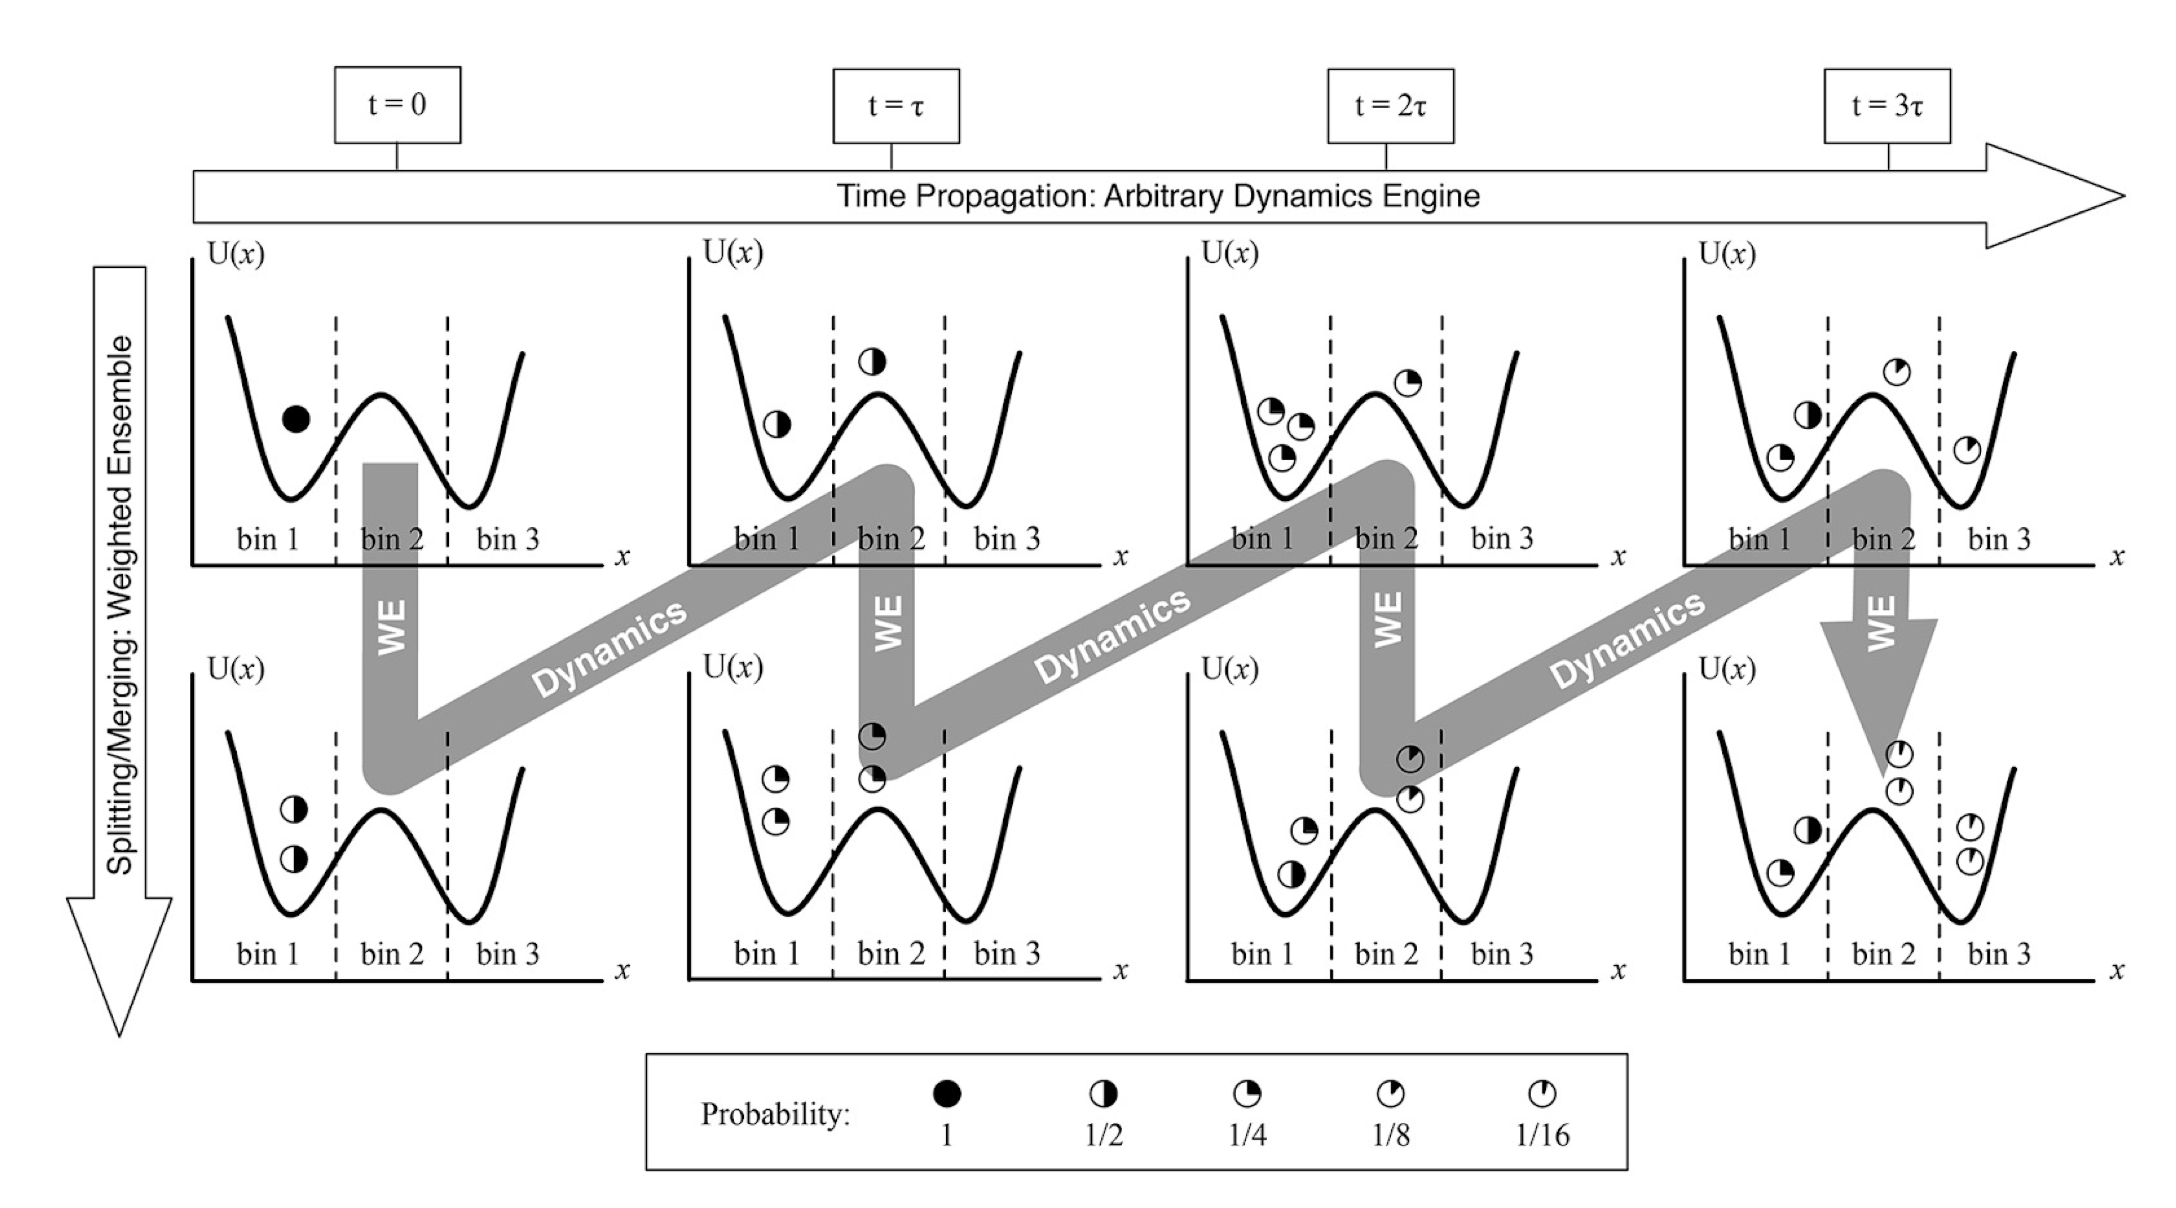
\includegraphics[width=\linewidth]{figure1_WE}
\caption{Overview of the weighted ensemble (WE) strategy \citep{donovan_unbiased_2016}.  WE typically employs bins, demarcated here by dashed vertical lines, to guide a set of trajectories to sample throughout configuration space.
Using only ordinary dynamics---without biasing forces---WE replicates (“splits”) trajectories in unoccupied or under-occupied regions of space and prunes (“merges”) trajectories in over-occupied regions, according to the user-specified allocation scheme which here is a target of two trajectories per bin.
Throughout the process, weights (partially filled circles) are tracked by statistical rules of inheritance that ensure that the overall ensemble dynamics are consistent with non-equilibrium statistical mechanics \citep{zhang_exact_2010}.
Figure adapted with permission from \citep{donovan_efficient_2013}.}
\end{figure*}

\subsection{The Weighted Ensemble Strategy}

WE is a highly-parallel path sampling strategy for generating rare events, for studying non-equilibrium steady states, and less commonly, for studying equilibrium properties. 
At heart, it is a simple and flexible strategy which is agnostic to system type and which therefore lends itself to numerous applications and optimizations. 
The properties of WE, including strengths and limitations, have been reviewed in detail before \citep{zuckerman_weighted_2017}, although improvements continue to be developed \citep{donyapour_revo_2019, copperman_accelerated_2020, torrillo_minimal_2021, degrave_red_2021, aristoff_optimizing_2020}. 
Here, we briefly review key aspects of WE.

\textbf{The Basic WE Procedure.} See \textbf{Figure 1}. 
WE orchestrates multiple trajectories---each assigned a weight---run in parallel by stopping them at regular time intervals of length $\tau$ (typically a large multiple of the underlying simulation time step), examining the trajectories, and restarting a new set of trajectories. 
The new trajectories are always continuations of the existing set, but some trajectories may not be continued (they are “pruned”) and others may be replicated. 
Discontinued trajectories result from probabilistic “merge” events where a continued trajectory absorbs the weight of one that is pruned. 
Replicated trajectories are said to be “split” with the original weight shared equally among the copies. 
Usually bins in configuration space are used to guide split and merge events based on a target number of trajectories for each bin, but any protocol---including binless strategies highlighted below---may be used for this purpose.
Regardless of the resampling protocol, a “recycling” protocol often is used whereby events reaching a user-specified target state are re-initiated according to a specified distribution of start states \citep{bhatt_steady-state_2010}.
This recycling protocol focuses all sampling on a single direction of a process of interest and has valuable properties as noted below.

\textbf{WE is Resampling, and Hence Unbiased.} The simple steps defining WE simulations stem from its basis as a statistical “resampling” procedure \citep{zhang_exact_2010}. 
The split/merge steps generate a statistically equivalent (re)sample of an initial trajectory set by increasing/reducing trajectory density in some regions of configuration space at a given time, using weight adjustments to maintain the underlying trajectory distribution. 
The trajectory set is therefore unbiased at all times, i.e., average time-dependent observables derived from many WE runs will match the average of a large number of conventional simulations without splitting or merging events \citep{zhang_exact_2010}. 
Furthermore, the distributions of transition path times (“barrier crossing times”) from WE runs match those from converged conventional simulations, and can be generated in orders of magnitude less computing time \citep{zwier_efficient_2011, zheng_simulating_2007}. 
The lack of bias in the dynamics of WE runs holds true regardless of whether recycling is employed.

\textbf{Observables and Ensembles Sampled by WE.} WE can yield transient and/or steady-state observables. 
When recycling is not used, WE provides pathways, i.e., sequences of conformations in a transition and the frequencies of those sequences, in addition to time-dependent observables as the system relaxes to equilibrium, e.g., the probability of a given event at a given time after initiation in the chosen starting state.
Complex systems are unlikely to relax fully to equilibrium during a WE simulation. 
With a recycling protocol, the system will not relax to equilibrium but instead to a non-equilibrium steady state (NESS) that has steady probability flow from initial to target state. 
If reached, the NESS provides a simple mechanism for computing rate constants via the Hill relation \citep{bhatt_steady-state_2010}. 
However, although relaxation to a NESS can be considerably faster than relaxation to equilibrium \citep{copperman_transient_2019,zuckerman_discrete-state_nodate}, the process may be too slow for WE to reach NESS on practical timescales, motivating the haMSM approach \citep{adhikari_computational_2019,copperman_accelerated_2020} described below.

\textbf{Resampling Introduces Correlations, which Increase Variance.} WE has intrinsic limitations, like any method \citep{chong_path-sampling_2017}, and it is essential to understand them. 
Most fundamentally, splitting and merging introduce correlations into the sampled trajectory ensemble that could decrease its information content. 
These stem primarily from splitting events: multiple trajectories share an identical history up to the time of the split event and hence do not contribute fully independent information to any observable.
These correlations, in turn, can lead to large run-to-run variance \citep{adhikari_computational_2019} because the trajectory ensemble in each WE run results from a relatively small number of “parent” trajectories which have been split repeatedly.
This variance is addressed to some extent by the iterative haMSM protocol described below, and more directly by ongoing mathematical optimizations noted below.  
Importantly, correlations within WE ensembles lead to significant challenges in quantifying uncertainty \citep{zuckerman_weighted_2017,mostofian_statistical_2019}.

\textbf{Ongiong Efforts at Optimization and Variance Reduction.} Because WE is unbiased so long as a correct resampling protocol is used \citep{zhang_exact_2010}, there is an opportunity to reduce the run-to-run variance noted above by improved resampling procedures. 
In the context of binned WE simulations, both the construction of bins and the number of trajectories per bin can be optimized based on a recently developed mathematical formulation \citep{aristoff_analysis_2018, aristoff_optimizing_2020} or based on heuristics \citep{torrillo_minimal_2021}. 
Bins do not need to be kept static over time \citep{zhang_exact_2010,dickson_wexplore_2014,torrillo_minimal_2021}. 
Optimization approaches are actively being studied and incorporated into WESTPA as appropriate.

\textbf{WE Cannot Solve Every Problem.} Despite its great strengths and highly notable achievements \citep{lotz_unbiased_2018, sztain_glycan_2021, adhikari_computational_2019}, users should not assume WE can tackle any problem.
Independent of the correlation/variance issues noted above, certain systems will remain too complex for WE given current hardware and algorithms.
In every system, there is a minimum transition path time t\textsubscript{TP} (also called t\textsubscript{b}) \citep{zuckerman_transition_2002, zhang_efficient_2007} for physically realistic events which sets an absolute requirement on sampling required: in a WE run, a set of trajectories exceeding the minimum t\textsubscript{TP} must be generated, which may be a prohibitive cost.
Additionally, even if the necessary computing resources are available, current binning and resampling strategies might not be sufficient to generate events of interest. 
And finally, even if events of interest are generated, the sampled trajectories may be insufficient for producing observables of interest such as a reliable estimate of the rate constant.

\subsection{Prerequisites}

\textbf{Background Knowledge and Experience.} All tutorials here are at the advanced level. 
Thus, a prerequisite for these tutorials is completion of the Basic and Intermediate WESTPA tutorials \citep{bogetti_suite_2019}, which have been updated for use with WESTPA version 2.0 ({\url{https://github.com/westpa/westpa_tutorials}}). 
Users should already have extensive experience running conventional simulations using the underlying dynamics engine of interest (Amber \citep{case_amber_2022}, OpenMM \citep{eastman_openmm_2017}, BioNetGen \citep{harris_bionetgen_2016}, etc.). 
Prior to applying the WE strategy to their own systems, we suggest that users run multiple conventional simulations to (i) ensure that the preparation of the system and propagation of dynamics is according to best practices (e.g., see \citep{braun_best_2019}), (ii) identify potential progress coordinates and initially define the target state, and (iii) estimate the ns/day on a single CPU/GPU for your system and storage needs for the full-scale WE simulation. 
We highly recommend that new WESTPA users read this review article \citep{zuckerman_weighted_2017} and this introduction to non-equilibrium physics of trajectories \citep{zuckerman_gentle_2021}. 

\textbf{Software Requirements.} The WESTPA 2.0 software is a standard Python package that can be used on any Unix operating system. 
The software requires Python versions $\geq$3.7 and a number of standard Python scientific computing packages. 
We recommend installing WESTPA either as a PyPI or conda package using miniconda. 
Both packages provide all required software dependencies and can be installed using one-line commands: (1) \verb|python -m pip install westpa| or (2) \verb|conda install -c conda-forge westpa|. 
Note that it is a best practice to install WESTPA into an isolated virtual or conda environment, along with the dependencies specific to your project. 
Due to the use of the MDTraj Python library with the WESTPA 2.0 HDF5 framework, certain modifications to the installation procedure are required for running WESTPA 2.0 on ppc64Ie architectures (e.g., TACC Longhorn or ORNL Summit supercomputers; see {\url{https://github.com/westpa/westpa/wiki/Alternate-Installation-Instructions}}). 

WESTPA 2.0 is designed to be interoperable with any dynamics engine, requiring an external dynamics engine to propagate the dynamics in a WE simulation.
Please see the prerequisite sections of each tutorial for additional software requirements that are specific to that tutorial.

\textbf{Hardware Requirements.} Like its predecessor, WESTPA 2.0 is highly-scalable on CPUs/GPUs, making optimal use of high-performance computing (HPC) clusters available at academic institutions or supercomputing centers. 
Memory requirements are dependent on the underlying dynamics engine, e.g., \textasciitilde1 GB per CPU core (or GPU) for atomistic MD simulations. 
Users should refer to the best practices of their dynamics engine of choice to determine the optimal allocation of resources for each CPU/GPU. 
The most efficient way to run WESTPA is to use a computing resource that provides the user with a number of CPUs/GPUs---all the same processor speed---that either matches the number of trajectories per WE iteration or a number by which the number of trajectories at any point in time is evenly divisible. 
WE can nevertheless run on heterogeneous hardware (different processor or memory bus speeds) or with trajectory counts that do not divide evenly onto CPUs/GPUs, but this scenario decreases efficiency as some processors are inevitably idle for at least a portion of the overall runtime.

Users can estimate the approximate storage space required for their project by taking the product of the following: (i) amount of disk space required for storing data from one trajectory segment of length $\tau$, (ii) the maximum number of trajectories per WE iteration, and (iii) the total number of WE iterations required to generate a reasonable maximum trajectory length. 
To optimize the use of storage space, we recommend that users tar up trajectory files into a single file for each WE iteration and remove coordinates of the system that are not of primary interest (e.g., solvent coordinates for certain processes). 
We note that the WESTPA 2.0 HDF5 framework dramatically reduces the storage space required for trajectory coordinates by consolidating the data from millions of small trajectory files into a relatively small number of larger HDF5 files, reducing the large overhead from the file system that results from the storage of numerous small trajectory files. 
By doing so, the HDF5 framework also alleviates potential I/O bottlenecks when a large amount of simulation files are written after each WE iteration. 